% Created 2018-11-15 Thu 14:56
% Intended LaTeX compiler: pdflatex
\documentclass[11pt]{article}
\usepackage[utf8]{inputenc}
\usepackage[T1]{fontenc}
\usepackage{graphicx}
\usepackage{grffile}
\usepackage{longtable}
\usepackage{wrapfig}
\usepackage{rotating}
\usepackage[normalem]{ulem}
\usepackage{amsmath}
\usepackage{textcomp}
\usepackage{amssymb}
\usepackage{capt-of}
\usepackage{hyperref}
\usepackage{minted}
\date{}
\title{}
\hypersetup{
 pdfauthor={Dinesh A},
 pdftitle={},
 pdfkeywords={},
 pdfsubject={},
 pdfcreator={Emacs 25.1.1 (Org mode 9.1.2)},
 pdflang={English}}
\begin{document}


\section{{\bfseries\sffamily TODO} Tests [1/3]}
\label{sec:orgcb56abb}
\subsection{{\bfseries\sffamily DONE} Case 1: No particles are overlapping}
\label{sec:org37dee35}
In this test case no particles are in contact. After executing the requisite
equations check for the contact indices of each particle. It has to be zero or
empty as expected.
\subsubsection{Create particles}
\label{sec:org86f6294}
\begin{minted}[]{sage}
# You can change the size of the image by providing the figsize argument.
import numpy as np
x = np.asarray([0., 0.21, -0.2, 0.2, 0.])
y = np.asarray([0., 0.21, 0.1, -0.1, 0.21])
R = np.ones_like(x) * 0.1

g = Graphics()
for i in range(len(x)):
    g += plot(circle((x[i], y[i]), R[i]))
    g += text(str(i), (x[i] + 0.01, y[i] + 0.01))
    g.show()
\end{minted}

\begin{center}
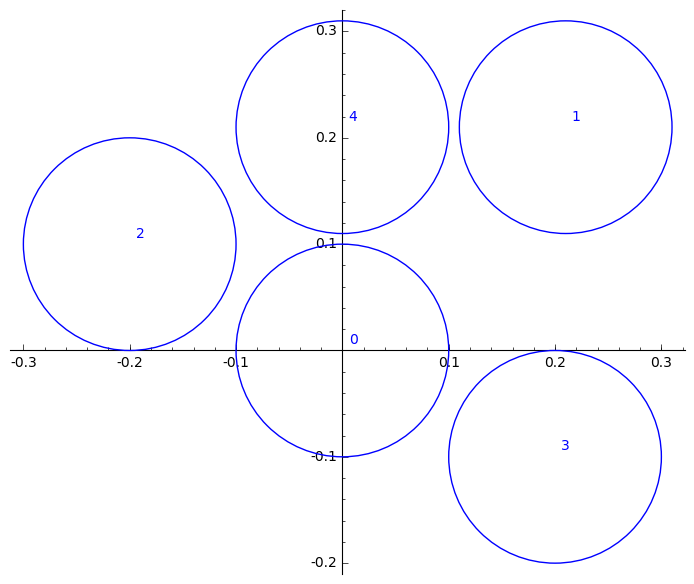
\includegraphics[width=.9\linewidth]{test_figures/test_case_1.png}
\end{center}

\subsubsection{Execute equations}
\label{sec:orgbbfcea2}
Now execute the linear force equation on the required particles.
\begin{minted}[]{python}
        # ------------------------------
        # execute the interparticle force equation
        # ------------------------------

        from pysph.tools.sph_evaluator import SPHEvaluator
        if self._sph_eval is None:
            equations = [
                LinearSpringForceParticleParticle(dest='sand',
                                                  sources=['sand'])
            ]

            self._sph_eval = SPHEvaluator(arrays=[self.pa],
                                          equations=equations, dim=2,
                                          kernel=CubicSpline(dim=2))

        self._sph_eval.evaluate()
\end{minted}
This equation has to add new contacts to the list and will \texttt{not} delete any
contacts if a particle is not overlapping. But if a particle is there in the
list but it is not overlapping then its tangential acceleration will be
zero.

\subsubsection{Check for contacts}
\label{sec:org83d8159}
Since in our case no particle is in contact with any other particle. After
executing the force equation the contact indices, contact displacements must
be as it is.

\begin{minted}[]{python}
        # check the tangential contacts indices and displacements
        # number of contacts of each individual particles
        for i in range(len(self.pa.x)):
            self.pa.total_tng_contacts[i] = 0.

        for i in range(self.pa.total_dem_entities[0]):
            self.pa.tng_idx[i] = -1
            self.pa.tng_x[i] = 0.
            self.pa.tng_y[i] = 0.
            self.pa.tng_z[i] = 0.
\end{minted}



\subsection{{\bfseries\sffamily TODO} Case 2: Add contacts}
\label{sec:orgb59afd7}
Create particles such that few of them are in contact. After executing the
equations the contacts will be updated. This will test the
\texttt{LinearSpringForce} equation. Now check the contact indices of each
particle. For an example say particle 1 is in overlap with 2, 5, 9. Then both
the particles tracking indices has to have their corresponding contacts in
the tracking history.


\subsubsection{Create particles}
\label{sec:orgeda8e99}
In this case make some particles to be in contact.
\begin{minted}[]{sage}
	# You can change the size of the image by providing the figsize argument.
import numpy as np
x = np.asarray([0., 0.21, -0.2, 0.2, 0.])
y = np.asarray([0., 0.21, 0.1, -0.1, 0.21])
R = np.ones_like(x) * 0.1

g = Graphics()
for i in range(len(x)):
    g += plot(circle((x[i], y[i]), R[i]))
    g += text(str(i), (x[i] + 0.01, y[i] + 0.01))
    g.show()
\end{minted}

\begin{center}
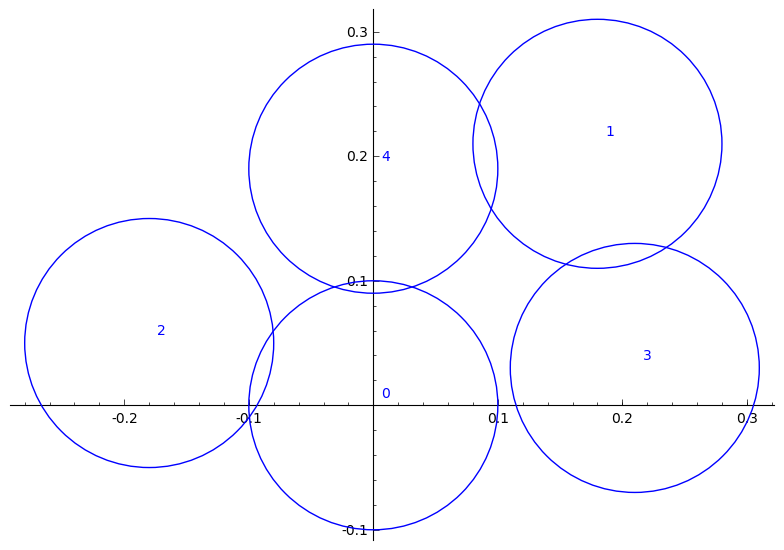
\includegraphics[width=.9\linewidth]{test_figures/test_case_2.png}
\end{center}

\subsubsection{Execute equations}
\label{sec:orgc1ba476}
\subsubsection{Check for contacts}
\label{sec:org66081ea}

\subsection{{\bfseries\sffamily TODO} Case 3: Remove contacts}
\label{sec:org9537e97}
Create particles such that only few are in contact. But the tracking indices
has to be more than the particles in contact. After executing the equations,
it has to remove the useless contact indices.

\subsubsection{Create particles}
\label{sec:orgdad66ea}
\subsubsection{Execute equations}
\label{sec:orgb8222bd}
\subsubsection{Check for contacts}
\label{sec:org9f366d9}
\end{document}